\documentclass{article}
\usepackage[english]{babel}
\usepackage[utf8]{inputenc}
\usepackage{fancyhdr}
\usepackage{geometry}
\usepackage{enumitem}
\usepackage{amsmath}
\usepackage{graphicx}
\usepackage{tcolorbox}
\usepackage{amssymb}
\usepackage[thinc]{esdiff}
\usepackage{float}

%%%%%%%%%%%%%%%%%%%%%%%%%%%%%%%%%%%%%%%%%%%%%%%%%%%%%%%%%%%%%%%%%%%%%%%%%%%%%%%% DOCUMENT FORMAT

\geometry{letterpaper, portrait, margin=1in}
\graphicspath{ {images/} }
\pagestyle{fancy}
\fancyhf{}
\lhead{Keerthik Muruganandam}
\rhead{Yadavalli Written Work 6}

%%%%%%%%%%%%%%%%%%%%%%%%%%%%%%%%%%%%%%%%%%%%%%%%%%%%%%%%%%%%%%%%%%%%%%%%%%%%%%%% BEGIN DOCUMENT

\begin{document}

\begin{enumerate}[label=\textbf{(6.\arabic*)}]

%%%%%%%%%%%%%%%%%%%%%%%%%%%%%%%%%%%%%%%%%%%%%%%%%%%%%%%%%%%%%%%%%%%%%%%%%%%%%%%% 7.1 PROBLEM STATEMENT

	\item Evaluate the area of the following graph
	\begin{figure}[H]
		\centering
		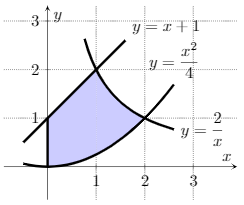
\includegraphics[scale=.75]{triginta}
		\caption{integral area}
	\end{figure}
%%%%%%%%%%%%%%%%%%%%%%%%%%%%%%%%%%%%%%%%%%%%%%%%%%%%%%%%%%%%%%%%%%%%%%%%%%% 7.1 WORK

To solve this, we can use the formula for area between two functions and apply it to the graph above. First, we must split our area into two parts, one from 0 to 1 and another from 1 to 2. Then, our top curves will be $x+1$ and $\dfrac{2}{x}$ for each limit respectively and our bottom curve will be $\dfrac{x^2}{4}$ for both integrals. Setting up what we have described yields
\[\int_0^1\!x+1-\frac{x^2}{4}\,dx+\int_1^2\!\frac{2}{x}-\frac{x^2}{4}\,dx\]
Computing the anti-derivatives of each integral using basic integration rules provides the expression
\[\left[\frac{x^2}{2}+x-\frac{x^3}{12}\right]_0^1+\left[2\ln|x|-\frac{x^2}{12}\right]_1^2\]
Now we can evaluate this to create the value
\begin{align*}
\left(\frac{1^2}{2}+1-\frac{1^3}{12}\right)-\left(\frac{0^2}{2}+0-\frac{0^3}{12}\right)+\left(2\ln|2|-\frac{2^2}{12}\right)-\left(1\ln|1|-\frac{1^1}{12}\right) &= \frac{1}{2}+1-\frac{1}{3}+\ln4 \\
&= \frac{11}{6}+\ln4
\end{align*}
That is the final value for our integral. Thus, the area of Figure 1 is equal to $\dfrac{11}{6}+\ln4$.

%%%%%%%%%%%%%%%%%%%%%%%%%%%%%%%%%%%%%%%%%%%%%%%%%%%%%%%%%%%%%%%%%%%%%%%%%%% NEWPAGE
\newpage
%%%%%%%%%%%%%%%%%%%%%%%%%%%%%%%%%%%%%%%%%%%%%%%%%%%%%%%%%%%%%%%%%%%%%%%%%%% 7.2 PROBLEM STATEMENT

\item Find the arc length of the graph of the function $y=\dfrac{e^x+e^{-x}}{2}$ over the interval $[0,3]$.
%%%%%%%%%%%%%%%%%%%%%%%%%%%%%%%%%%%%%%%%%%%%%%%%%%%%%%%%%%%%%%%%%%%%%%%%%%% 7.2 WORK

First of all, recall the arc length equation, which is to find the length of a function $f(x)$ on $[a,b]$
\[L=\int_a^b\!\sqrt{1+\left(f^\prime(x)\right)^2}\,dx\]
Now let $f(x)=\dfrac{e^x+e^{-x}}{2}$ and $[a,b]=[0,3]$. Computing the derivative of $f(x)$ is accomplished by using derivative rules.
\begin{align*}
\diff{}{x}\left(\frac{e^x+e^{-x}}{2}\right) &= \frac{1}{2}\diff{}{x}\left(e^x+e^{-x}\right)\\
&= \frac{1}{2}(e^x-e^{-x})
\end{align*}
The equation for the arc length is then
\begin{align*}
L &= \int_0^3\!\sqrt{1+\left(\frac{1}{2}(e^x-e^{-x})\right)^2}\,dx \\
&= \int_0^3\!\sqrt{\frac{e^{2x}+2+e^{-2x}}{4}}\,dx
\end{align*}
This integral is not easily computable by hand. 

%%%%%%%%%%%%%%%%%%%%%%%%%%%%%%%%%%%%%%%%%%%%%%%%%%%%%%%%%%%%%%%%%%%%%%%%%%% END DOCUMENT

\end{enumerate}
\end{document}
